\documentclass[]{article}
\usepackage{lmodern}
\usepackage{amssymb,amsmath}
\usepackage{ifxetex,ifluatex}
\usepackage{fixltx2e} % provides \textsubscript
\ifnum 0\ifxetex 1\fi\ifluatex 1\fi=0 % if pdftex
  \usepackage[T1]{fontenc}
  \usepackage[utf8]{inputenc}
\else % if luatex or xelatex
  \ifxetex
    \usepackage{mathspec}
  \else
    \usepackage{fontspec}
  \fi
  \defaultfontfeatures{Ligatures=TeX,Scale=MatchLowercase}
\fi
% use upquote if available, for straight quotes in verbatim environments
\IfFileExists{upquote.sty}{\usepackage{upquote}}{}
% use microtype if available
\IfFileExists{microtype.sty}{%
\usepackage{microtype}
\UseMicrotypeSet[protrusion]{basicmath} % disable protrusion for tt fonts
}{}
\usepackage[margin=1in]{geometry}
\usepackage{hyperref}
\hypersetup{unicode=true,
            pdftitle={Statistical inference},
            pdfauthor={saurabh yadav},
            pdfborder={0 0 0},
            breaklinks=true}
\urlstyle{same}  % don't use monospace font for urls
\usepackage{color}
\usepackage{fancyvrb}
\newcommand{\VerbBar}{|}
\newcommand{\VERB}{\Verb[commandchars=\\\{\}]}
\DefineVerbatimEnvironment{Highlighting}{Verbatim}{commandchars=\\\{\}}
% Add ',fontsize=\small' for more characters per line
\usepackage{framed}
\definecolor{shadecolor}{RGB}{248,248,248}
\newenvironment{Shaded}{\begin{snugshade}}{\end{snugshade}}
\newcommand{\KeywordTok}[1]{\textcolor[rgb]{0.13,0.29,0.53}{\textbf{#1}}}
\newcommand{\DataTypeTok}[1]{\textcolor[rgb]{0.13,0.29,0.53}{#1}}
\newcommand{\DecValTok}[1]{\textcolor[rgb]{0.00,0.00,0.81}{#1}}
\newcommand{\BaseNTok}[1]{\textcolor[rgb]{0.00,0.00,0.81}{#1}}
\newcommand{\FloatTok}[1]{\textcolor[rgb]{0.00,0.00,0.81}{#1}}
\newcommand{\ConstantTok}[1]{\textcolor[rgb]{0.00,0.00,0.00}{#1}}
\newcommand{\CharTok}[1]{\textcolor[rgb]{0.31,0.60,0.02}{#1}}
\newcommand{\SpecialCharTok}[1]{\textcolor[rgb]{0.00,0.00,0.00}{#1}}
\newcommand{\StringTok}[1]{\textcolor[rgb]{0.31,0.60,0.02}{#1}}
\newcommand{\VerbatimStringTok}[1]{\textcolor[rgb]{0.31,0.60,0.02}{#1}}
\newcommand{\SpecialStringTok}[1]{\textcolor[rgb]{0.31,0.60,0.02}{#1}}
\newcommand{\ImportTok}[1]{#1}
\newcommand{\CommentTok}[1]{\textcolor[rgb]{0.56,0.35,0.01}{\textit{#1}}}
\newcommand{\DocumentationTok}[1]{\textcolor[rgb]{0.56,0.35,0.01}{\textbf{\textit{#1}}}}
\newcommand{\AnnotationTok}[1]{\textcolor[rgb]{0.56,0.35,0.01}{\textbf{\textit{#1}}}}
\newcommand{\CommentVarTok}[1]{\textcolor[rgb]{0.56,0.35,0.01}{\textbf{\textit{#1}}}}
\newcommand{\OtherTok}[1]{\textcolor[rgb]{0.56,0.35,0.01}{#1}}
\newcommand{\FunctionTok}[1]{\textcolor[rgb]{0.00,0.00,0.00}{#1}}
\newcommand{\VariableTok}[1]{\textcolor[rgb]{0.00,0.00,0.00}{#1}}
\newcommand{\ControlFlowTok}[1]{\textcolor[rgb]{0.13,0.29,0.53}{\textbf{#1}}}
\newcommand{\OperatorTok}[1]{\textcolor[rgb]{0.81,0.36,0.00}{\textbf{#1}}}
\newcommand{\BuiltInTok}[1]{#1}
\newcommand{\ExtensionTok}[1]{#1}
\newcommand{\PreprocessorTok}[1]{\textcolor[rgb]{0.56,0.35,0.01}{\textit{#1}}}
\newcommand{\AttributeTok}[1]{\textcolor[rgb]{0.77,0.63,0.00}{#1}}
\newcommand{\RegionMarkerTok}[1]{#1}
\newcommand{\InformationTok}[1]{\textcolor[rgb]{0.56,0.35,0.01}{\textbf{\textit{#1}}}}
\newcommand{\WarningTok}[1]{\textcolor[rgb]{0.56,0.35,0.01}{\textbf{\textit{#1}}}}
\newcommand{\AlertTok}[1]{\textcolor[rgb]{0.94,0.16,0.16}{#1}}
\newcommand{\ErrorTok}[1]{\textcolor[rgb]{0.64,0.00,0.00}{\textbf{#1}}}
\newcommand{\NormalTok}[1]{#1}
\usepackage{graphicx,grffile}
\makeatletter
\def\maxwidth{\ifdim\Gin@nat@width>\linewidth\linewidth\else\Gin@nat@width\fi}
\def\maxheight{\ifdim\Gin@nat@height>\textheight\textheight\else\Gin@nat@height\fi}
\makeatother
% Scale images if necessary, so that they will not overflow the page
% margins by default, and it is still possible to overwrite the defaults
% using explicit options in \includegraphics[width, height, ...]{}
\setkeys{Gin}{width=\maxwidth,height=\maxheight,keepaspectratio}
\IfFileExists{parskip.sty}{%
\usepackage{parskip}
}{% else
\setlength{\parindent}{0pt}
\setlength{\parskip}{6pt plus 2pt minus 1pt}
}
\setlength{\emergencystretch}{3em}  % prevent overfull lines
\providecommand{\tightlist}{%
  \setlength{\itemsep}{0pt}\setlength{\parskip}{0pt}}
\setcounter{secnumdepth}{0}
% Redefines (sub)paragraphs to behave more like sections
\ifx\paragraph\undefined\else
\let\oldparagraph\paragraph
\renewcommand{\paragraph}[1]{\oldparagraph{#1}\mbox{}}
\fi
\ifx\subparagraph\undefined\else
\let\oldsubparagraph\subparagraph
\renewcommand{\subparagraph}[1]{\oldsubparagraph{#1}\mbox{}}
\fi

%%% Use protect on footnotes to avoid problems with footnotes in titles
\let\rmarkdownfootnote\footnote%
\def\footnote{\protect\rmarkdownfootnote}

%%% Change title format to be more compact
\usepackage{titling}

% Create subtitle command for use in maketitle
\newcommand{\subtitle}[1]{
  \posttitle{
    \begin{center}\large#1\end{center}
    }
}

\setlength{\droptitle}{-2em}

  \title{Statistical inference}
    \pretitle{\vspace{\droptitle}\centering\huge}
  \posttitle{\par}
    \author{saurabh yadav}
    \preauthor{\centering\large\emph}
  \postauthor{\par}
      \predate{\centering\large\emph}
  \postdate{\par}
    \date{19 August 2018}


\begin{document}
\maketitle

\subsection{A Simulation Excersise}\label{a-simulation-excersise}

\paragraph{Simulating exponantial
variables}\label{simulating-exponantial-variables}

\begin{Shaded}
\begin{Highlighting}[]
\KeywordTok{library}\NormalTok{(ggplot2)}
\end{Highlighting}
\end{Shaded}

\begin{verbatim}
## Warning: package 'ggplot2' was built under R version 3.5.1
\end{verbatim}

\begin{Shaded}
\begin{Highlighting}[]
\NormalTok{n<-}\DecValTok{1000}
\NormalTok{col<-}\DecValTok{40}
\NormalTok{expovar<-}\KeywordTok{rexp}\NormalTok{(n}\OperatorTok{*}\NormalTok{col,}\FloatTok{0.2}\NormalTok{)}
\end{Highlighting}
\end{Shaded}

\paragraph{creating matrix for the exponantial
variables}\label{creating-matrix-for-the-exponantial-variables}

\begin{Shaded}
\begin{Highlighting}[]
\NormalTok{mat<-}\KeywordTok{matrix}\NormalTok{(expovar,n,col)}
\end{Highlighting}
\end{Shaded}

\paragraph{taking the mean of the 40 exponantial
variables}\label{taking-the-mean-of-the-40-exponantial-variables}

\begin{Shaded}
\begin{Highlighting}[]
\NormalTok{expomean<-}\KeywordTok{apply}\NormalTok{(mat, }\DecValTok{1}\NormalTok{, mean)}
\end{Highlighting}
\end{Shaded}

\subsubsection{Comparisons}\label{comparisons}

\paragraph{Comparison between sample mean and the theoretical
mean}\label{comparison-between-sample-mean-and-the-theoretical-mean}

\paragraph{1.mean of the population}\label{mean-of-the-population}

\begin{Shaded}
\begin{Highlighting}[]
\KeywordTok{mean}\NormalTok{(expovar)}
\end{Highlighting}
\end{Shaded}

\begin{verbatim}
## [1] 4.986686
\end{verbatim}

\paragraph{plotting the distribution of
averages}\label{plotting-the-distribution-of-averages}

\begin{Shaded}
\begin{Highlighting}[]
\KeywordTok{ggplot}\NormalTok{()}\OperatorTok{+}\KeywordTok{geom_histogram}\NormalTok{(}\KeywordTok{aes}\NormalTok{(expomean),}\DataTypeTok{col=}\StringTok{"black"}\NormalTok{,}\DataTypeTok{fill=}\StringTok{"steelblue"}\NormalTok{)}\OperatorTok{+}\KeywordTok{geom_density}\NormalTok{()}\OperatorTok{+}\KeywordTok{geom_vline}\NormalTok{(}\KeywordTok{aes}\NormalTok{(}\DataTypeTok{xintercept=}\KeywordTok{mean}\NormalTok{(expomean, }\DataTypeTok{na.rm=}\NormalTok{T)))}\OperatorTok{+}\KeywordTok{labs}\NormalTok{(}\DataTypeTok{x=}\StringTok{"averages of 40 variables"}\NormalTok{)}
\end{Highlighting}
\end{Shaded}

\begin{verbatim}
## `stat_bin()` using `bins = 30`. Pick better value with `binwidth`.
\end{verbatim}

\includegraphics{inference_files/figure-latex/unnamed-chunk-5-1.pdf}
\#\#\#RESULT

\paragraph{The plot shows the distribution of averages is normally
distributed and follows the Central Limit
Theorm}\label{the-plot-shows-the-distribution-of-averages-is-normally-distributed-and-follows-the-central-limit-theorm}

\paragraph{The population mean and the mean of averages are approximate
beacause the plot is centered around the population
mean}\label{the-population-mean-and-the-mean-of-averages-are-approximate-beacause-the-plot-is-centered-around-the-population-mean}

\subsection{PART-2 Basic inferential data
analysis}\label{part-2-basic-inferential-data-analysis}

\paragraph{Loading the tooth data}\label{loading-the-tooth-data}

\begin{Shaded}
\begin{Highlighting}[]
\KeywordTok{data}\NormalTok{(}\StringTok{"ToothGrowth"}\NormalTok{)}
\end{Highlighting}
\end{Shaded}

\paragraph{Subsetting the tooth growth data on the basis of the
supp}\label{subsetting-the-tooth-growth-data-on-the-basis-of-the-supp}

\begin{Shaded}
\begin{Highlighting}[]
\NormalTok{vc<-}\KeywordTok{subset}\NormalTok{(ToothGrowth,supp}\OperatorTok{==}\StringTok{"VC"}\NormalTok{)}
\NormalTok{oj<-}\KeywordTok{subset}\NormalTok{(ToothGrowth,supp}\OperatorTok{==}\StringTok{"OJ"}\NormalTok{)}
\end{Highlighting}
\end{Shaded}

\paragraph{Arranging the datasets on the basis of
doses}\label{arranging-the-datasets-on-the-basis-of-doses}

\begin{Shaded}
\begin{Highlighting}[]
\NormalTok{newvc<-}\KeywordTok{c}\NormalTok{()}
\NormalTok{newvc}\OperatorTok{$}\NormalTok{dose0.}\DecValTok{5}\NormalTok{<-vc}\OperatorTok{$}\NormalTok{len[vc}\OperatorTok{$}\NormalTok{dose}\OperatorTok{==}\FloatTok{0.5}\NormalTok{]}
\NormalTok{newvc}\OperatorTok{$}\NormalTok{dose1<-vc}\OperatorTok{$}\NormalTok{len[vc}\OperatorTok{$}\NormalTok{dose}\OperatorTok{==}\DecValTok{1}\NormalTok{]}
\NormalTok{newvc}\OperatorTok{$}\NormalTok{dose2<-vc}\OperatorTok{$}\NormalTok{len[vc}\OperatorTok{$}\NormalTok{dose}\OperatorTok{==}\DecValTok{2}\NormalTok{]}
\NormalTok{newvc<-}\KeywordTok{data.frame}\NormalTok{(newvc)}
\NormalTok{newoj<-}\KeywordTok{c}\NormalTok{()}
\NormalTok{newoj}\OperatorTok{$}\NormalTok{dose0.}\DecValTok{5}\NormalTok{<-oj}\OperatorTok{$}\NormalTok{len[oj}\OperatorTok{$}\NormalTok{dose}\OperatorTok{==}\FloatTok{0.5}\NormalTok{]}
\NormalTok{newoj}\OperatorTok{$}\NormalTok{dose1<-oj}\OperatorTok{$}\NormalTok{len[oj}\OperatorTok{$}\NormalTok{dose}\OperatorTok{==}\DecValTok{1}\NormalTok{]}
\NormalTok{newoj}\OperatorTok{$}\NormalTok{dose2<-oj}\OperatorTok{$}\NormalTok{len[oj}\OperatorTok{$}\NormalTok{dose}\OperatorTok{==}\DecValTok{2}\NormalTok{]}
\NormalTok{newoj<-}\KeywordTok{data.frame}\NormalTok{(newoj)}
\end{Highlighting}
\end{Shaded}

\paragraph{Taking the mean of the length of the tooth growth for
different
doses}\label{taking-the-mean-of-the-length-of-the-tooth-growth-for-different-doses}

\begin{Shaded}
\begin{Highlighting}[]
\NormalTok{lengthmeanvc<-}\KeywordTok{apply}\NormalTok{(newvc, }\DecValTok{2}\NormalTok{, mean)}
\NormalTok{lengthmeanoj<-}\KeywordTok{apply}\NormalTok{(newoj, }\DecValTok{2}\NormalTok{, mean)}
\end{Highlighting}
\end{Shaded}

\paragraph{converting it into a marix}\label{converting-it-into-a-marix}

\begin{Shaded}
\begin{Highlighting}[]
\NormalTok{lengthmeanvc<-}\KeywordTok{data.frame}\NormalTok{(}\KeywordTok{matrix}\NormalTok{(lengthmeanvc))}
\NormalTok{lengthmeanoj<-}\KeywordTok{data.frame}\NormalTok{(}\KeywordTok{matrix}\NormalTok{(lengthmeanoj))}
\end{Highlighting}
\end{Shaded}

\paragraph{giving new column names}\label{giving-new-column-names}

\begin{Shaded}
\begin{Highlighting}[]
\KeywordTok{colnames}\NormalTok{(lengthmeanvc)<-}\StringTok{"len"}
\KeywordTok{rownames}\NormalTok{(lengthmeanvc)<-}\KeywordTok{c}\NormalTok{(}\StringTok{"dose0.5"}\NormalTok{,}\StringTok{"dose1"}\NormalTok{,}\StringTok{"dose2"}\NormalTok{)}
\KeywordTok{colnames}\NormalTok{(lengthmeanoj)<-}\StringTok{"len"}
\KeywordTok{rownames}\NormalTok{(lengthmeanoj)<-}\KeywordTok{c}\NormalTok{(}\StringTok{"dose0.5"}\NormalTok{,}\StringTok{"dose1"}\NormalTok{,}\StringTok{"dose2"}\NormalTok{)}
\end{Highlighting}
\end{Shaded}

\paragraph{adding new coloumn}\label{adding-new-coloumn}

\begin{Shaded}
\begin{Highlighting}[]
\NormalTok{lengthmeanvc}\OperatorTok{$}\NormalTok{dose<-}\KeywordTok{c}\NormalTok{(}\FloatTok{0.5}\NormalTok{,}\DecValTok{1}\NormalTok{,}\DecValTok{2}\NormalTok{)}
\NormalTok{lengthmeanoj}\OperatorTok{$}\NormalTok{dose<-}\KeywordTok{c}\NormalTok{(}\FloatTok{0.5}\NormalTok{,}\DecValTok{1}\NormalTok{,}\DecValTok{2}\NormalTok{)}
\end{Highlighting}
\end{Shaded}

\paragraph{plotting}\label{plotting}

\begin{Shaded}
\begin{Highlighting}[]
\NormalTok{len<-lengthmeanvc}
\KeywordTok{colnames}\NormalTok{(len)<-}\KeywordTok{c}\NormalTok{(}\StringTok{"lenVC"}\NormalTok{,}\StringTok{"dose"}\NormalTok{)}
\NormalTok{len}\OperatorTok{$}\NormalTok{lenOJ<-lengthmeanoj}\OperatorTok{$}\NormalTok{len}
\end{Highlighting}
\end{Shaded}

\paragraph{plotting'}\label{plotting-1}

\begin{Shaded}
\begin{Highlighting}[]
\KeywordTok{ggplot}\NormalTok{(len,}\KeywordTok{aes}\NormalTok{(dose,lenVC))}\OperatorTok{+}\KeywordTok{geom_line}\NormalTok{(}\DataTypeTok{color=}\StringTok{"steelblue"}\NormalTok{)}\OperatorTok{+}\KeywordTok{geom_point}\NormalTok{(}\DataTypeTok{color=}\StringTok{"blue"}\NormalTok{)}\OperatorTok{+}\KeywordTok{geom_point}\NormalTok{(}\KeywordTok{aes}\NormalTok{(dose,lenOJ))}\OperatorTok{+}\KeywordTok{geom_line}\NormalTok{(}\KeywordTok{aes}\NormalTok{(dose,lenOJ),}\DataTypeTok{color=}\StringTok{"red"}\NormalTok{)}\OperatorTok{+}\KeywordTok{labs}\NormalTok{(}\DataTypeTok{title=}\StringTok{"effect of doses of different supplies on tooth growth"}\NormalTok{)}\OperatorTok{+}\KeywordTok{labs}\NormalTok{(}\DataTypeTok{x=}\StringTok{"DOSES"}\NormalTok{,}\DataTypeTok{y=}\StringTok{"length"}\NormalTok{)}\OperatorTok{+}\KeywordTok{geom_point}\NormalTok{(}\KeywordTok{aes}\NormalTok{(dose,lenOJ),}\DataTypeTok{color=}\StringTok{"red"}\NormalTok{)}
\end{Highlighting}
\end{Shaded}

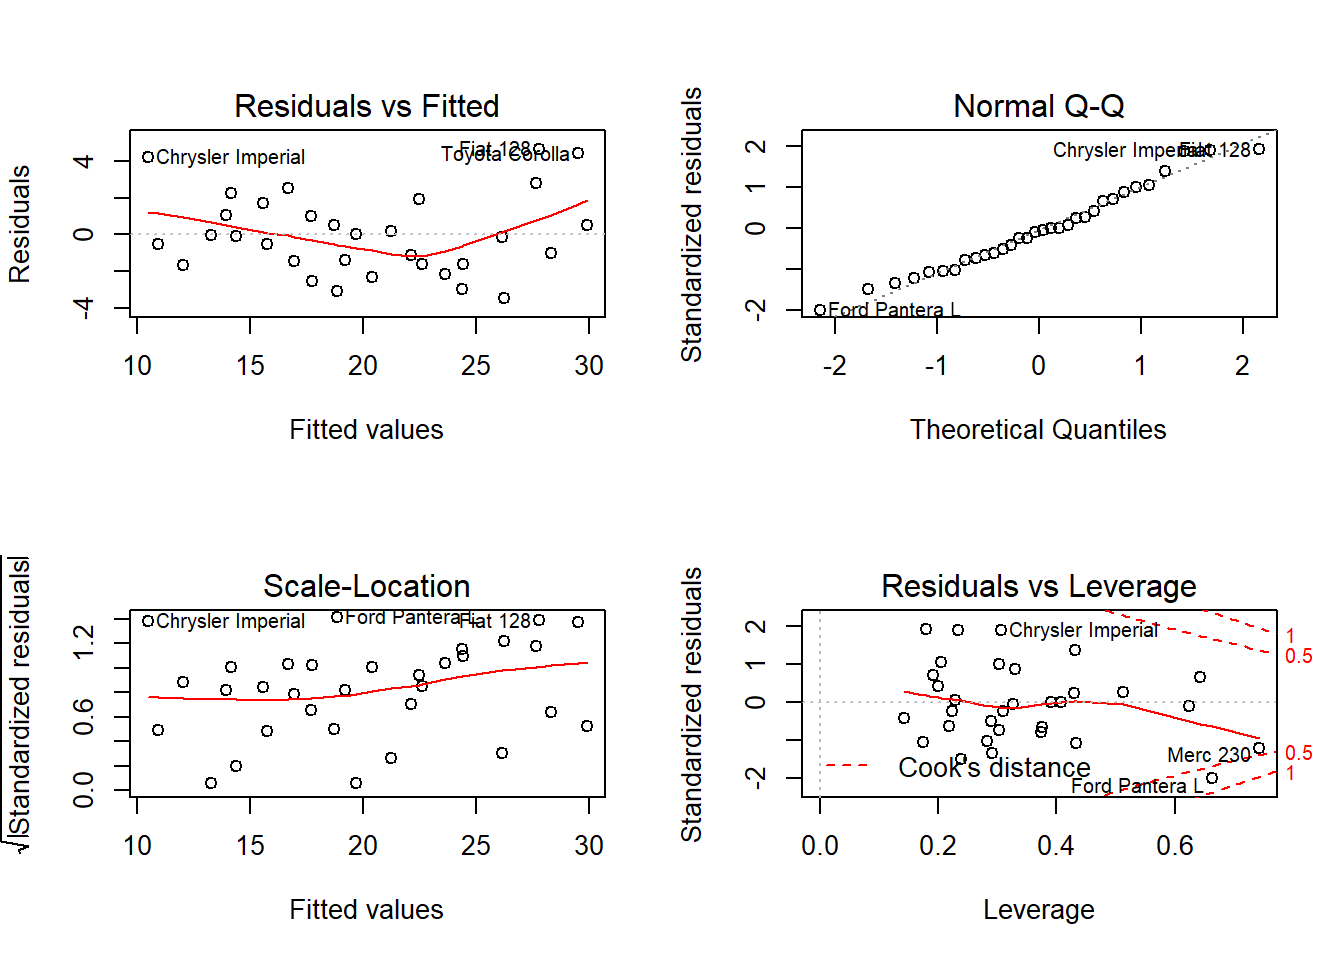
\includegraphics{inference_files/figure-latex/unnamed-chunk-14-1.pdf}

\paragraph{Using confidence intervals and/or hypothesis tests to compare
tooth growth by supp and
dose}\label{using-confidence-intervals-andor-hypothesis-tests-to-compare-tooth-growth-by-supp-and-dose}

\paragraph{Confidence interval for dose
0.5}\label{confidence-interval-for-dose-0.5}

\begin{Shaded}
\begin{Highlighting}[]
\KeywordTok{t.test}\NormalTok{(oj}\OperatorTok{$}\NormalTok{len[oj}\OperatorTok{$}\NormalTok{dose}\OperatorTok{==}\FloatTok{0.5}\NormalTok{],vc}\OperatorTok{$}\NormalTok{len[vc}\OperatorTok{$}\NormalTok{dose}\OperatorTok{==}\FloatTok{0.5}\NormalTok{],}\DataTypeTok{paired =}\NormalTok{ F)}\OperatorTok{$}\NormalTok{conf.int}
\end{Highlighting}
\end{Shaded}

\begin{verbatim}
## [1] 1.719057 8.780943
## attr(,"conf.level")
## [1] 0.95
\end{verbatim}

\subsubsection{RESULT: The t test between the supp vc and oj for
dose=0.5 gives the interval 1.719057 to 8.780943. Which means the dose
of 0.5 for oj is way more effective for tooth
growth.}\label{result-the-t-test-between-the-supp-vc-and-oj-for-dose0.5-gives-the-interval-1.719057-to-8.780943.-which-means-the-dose-of-0.5-for-oj-is-way-more-effective-for-tooth-growth.}

\paragraph{Confidence interval for dose
1}\label{confidence-interval-for-dose-1}

\begin{Shaded}
\begin{Highlighting}[]
\KeywordTok{t.test}\NormalTok{(oj}\OperatorTok{$}\NormalTok{len[oj}\OperatorTok{$}\NormalTok{dose}\OperatorTok{==}\DecValTok{1}\NormalTok{],vc}\OperatorTok{$}\NormalTok{len[vc}\OperatorTok{$}\NormalTok{dose}\OperatorTok{==}\DecValTok{1}\NormalTok{],}\DataTypeTok{paired =}\NormalTok{ F)}\OperatorTok{$}\NormalTok{conf.int}
\end{Highlighting}
\end{Shaded}

\begin{verbatim}
## [1] 2.802148 9.057852
## attr(,"conf.level")
## [1] 0.95
\end{verbatim}

\subsubsection{RESULT: The t test between the supp vc and oj for dose=1
gives the interval 2.802148 to 9.057852. Which means the dose of 1 for
oj is way more effective for tooth
growth.}\label{result-the-t-test-between-the-supp-vc-and-oj-for-dose1-gives-the-interval-2.802148-to-9.057852.-which-means-the-dose-of-1-for-oj-is-way-more-effective-for-tooth-growth.}

\paragraph{Confidence interval for dose
2}\label{confidence-interval-for-dose-2}

\begin{Shaded}
\begin{Highlighting}[]
\KeywordTok{t.test}\NormalTok{(oj}\OperatorTok{$}\NormalTok{len[oj}\OperatorTok{$}\NormalTok{dose}\OperatorTok{==}\DecValTok{2}\NormalTok{],vc}\OperatorTok{$}\NormalTok{len[vc}\OperatorTok{$}\NormalTok{dose}\OperatorTok{==}\DecValTok{2}\NormalTok{],}\DataTypeTok{paired =}\NormalTok{ F)}\OperatorTok{$}\NormalTok{conf.int}
\end{Highlighting}
\end{Shaded}

\begin{verbatim}
## [1] -3.79807  3.63807
## attr(,"conf.level")
## [1] 0.95
\end{verbatim}

\subsubsection{RESULT: The t test between the supp vc and oj for dose=2
gives the interval -3.79807 to 3.63807. Which means the dose of 2 for
both vc and oj are approximately same. This can also be shown by the
plot which clearly shows that dose 2 for both affect the tooth growth in
a same
way.}\label{result-the-t-test-between-the-supp-vc-and-oj-for-dose2-gives-the-interval--3.79807-to-3.63807.-which-means-the-dose-of-2-for-both-vc-and-oj-are-approximately-same.-this-can-also-be-shown-by-the-plot-which-clearly-shows-that-dose-2-for-both-affect-the-tooth-growth-in-a-same-way.}

\subsubsection{Conclusion}\label{conclusion}

\paragraph{The effect of two medications are similar when the dose is
2.}\label{the-effect-of-two-medications-are-similar-when-the-dose-is-2.}

\paragraph{The oj is more effective in tooth growth when the doses are
0.5 and
1}\label{the-oj-is-more-effective-in-tooth-growth-when-the-doses-are-0.5-and-1}


\end{document}
